\documentclass{standalone}
\usepackage{tikz}

\usetikzlibrary{calc,math}


\begin{document}

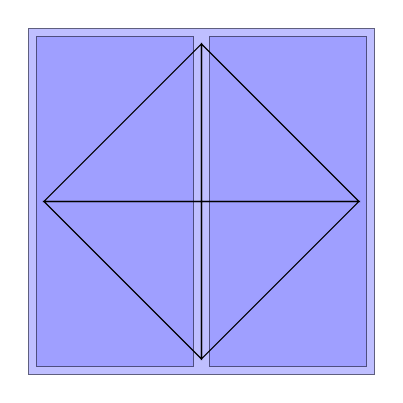
\begin{tikzpicture}
  \tikzmath{
    real \radius;
    \radius = 2;
  }

  \draw[fill=blue!50,opacity=.5] (-\radius*1.1,-\radius*1.1) rectangle (\radius*1.1,\radius*1.1);
  \draw[fill=blue!50,opacity=.5] (-\radius*1.05,-\radius*1.05) rectangle (-\radius*0.05,\radius*1.05);
  \draw[fill=blue!50,opacity=.5] (\radius*0.05,-\radius*1.05) rectangle (\radius*1.05,\radius*1.05);

  \foreach[evaluate={\i + 90} as \j] \i in {0,90,...,270} {
    \draw (0,0) -- (\i:\radius) -- (\j:\radius) -- cycle;
  }
\end{tikzpicture}

\end{document}